\chapter{Internal specification}

\begin{itemize}
\item concept of the system
\item system architecture
\item description of data structures (and data bases)
\item components, modules, libraries, resume of important classes (if used)
\item resume of important algorithms (if used)
\item details of implementation of selected parts
\item applied design patterns
\item UML diagrams
\end{itemize}

\section{Documentation}

This section consists of variables that are used later in the project. By changing these values, modification of the application is possible. All variables that matter are stored here. company{\_}name and price{\_}type are used in reading data from Yahoo Finance. In company{\_}name, the NASDAQ (National Association of Securities Dealers Automated Quotations) ticker symbol should be imputed so that the appropriate company data could be read. The ticker symbol is an abbreviation of the company name used in NASDAQ to associate a particular company with its data. In price{\_}type, the type of price that should be read should be specified from open price (open), closing price (close), the highest price of the given period of time (high), lowest price of the given period of time (low) or the volume traded (volume).

\clearpage
\begin{figure}
\centering
\begin{lstlisting}
  # Variables
  company_name = 'GOOGL' # company NASDAQ name
  price_type = 'open' # open, close, high, low, volume
  
  
  # Time interval
  startDate = '2021-06-01'
  endDate = '2022-06-01'
  interval = 'daily' # daily, weekly or monthly
  
  
  # Shape of input data
  chunkSize = 20
\end{lstlisting}
\caption{Variables.}
\label{fig:pseudocode:listings}
\end{figure}

YahooFinancials is easy to use and outputs raw data that can be conveniently used later. data{\_}price{\_}raw stores all data of a given company in the time period between startDate and endDate in chosen intervals. data{\_}prices stores only the prices without the index of date, name, et cetera.
Two ‘for loops’ append the data to the arrays created earlier. The data is assigned so that the neural network’s input data is the chosen number of days, and the test data is the next day so that the next day can be predicted on the chosen number of the days before it. For example, for chosen 30 days, the input data are 29 days, and the output should be the one next day (29:1).

\clearpage
\begin{figure}
\centering
\begin{lstlisting}
  yahoo_financials = YahooFinancials(company_name)
  data_prices_raw = yahoo_financials.get_historical_price_data(startDate, endDate, interval)
  data_prices = data_prices_raw[company_name]['prices']
  
  
  for i in range(len(data_prices)):
   data.append(data_prices[i][price_type])
  
  
  for i in range(chunkSize, len(data_prices) - 1):
   data_prediction.append(data[i-chunkSize:i])
   data_result.append(data[i])
\end{lstlisting}
\caption{Working with the stock market data.}
\label{fig:pseudocode:listings}
\end{figure}

In order to train the model, the gathered data should be reshaped so that they have three dimensions. This operation can be done with a few arithmetic operations, but it is more convenient to use reliable methods to do so. Firstly, the given data is transformed with minmax{\_}scale() to normalize the data between 0 and 0.999. Then using the numpy reshape() function, the data is reshaped into three dimensions.

\clearpage
\begin{figure}
\centering
\begin{lstlisting}
  # Reshape the data
  # into 3 dimensions
  data_result, data_prediction = np.array(data_result), np.array(data_prediction)
  
  
  data_prediction = minmax_scale(data_prediction, feature_range=(0,.999))
  data_prediction = np.reshape(data_prediction, (data_prediction.shape[0], data_prediction.shape[1], 1))
  data_result = minmax_scale(data_result, feature_range=(0,.999)
\end{lstlisting}
\caption{Reshaping data.}
\label{fig:pseudocode:listings}
\end{figure}

As it was stated before in this paper, the chosen type of model for this project is the Sequential model, as it was proven to work best for such solutions in different papers. In this project, several combinations of different layers have been considered, and finally, the layers presented below have been added to the model.
\par

LSTM -> Dropout -> LSTM -> Dropout -> Dense
\clearpage
\begin{figure}
\centering
\begin{lstlisting}
  model = Sequential()
  model.add(LSTM(50, return_sequences=True, input_shape=(data_prediction.shape[1], 1)))
  model.add(Dropout(0.2))
  model.add(LSTM(50, return_sequences=False))
  model.add(Dropout(0.2))
  model.add(Dense(1))
\end{lstlisting}
\caption{Neural network model.}
\label{fig:pseudocode:listings}
\end{figure}

The model has been compiled using the ‘adam’ optimizer, and for loss, ‘mean squared error’ has been used.
\clearpage
\begin{figure}
\centering
\begin{lstlisting}
  model.compile(optimizer='adam',
  loss='mean_squared_error')
\end{lstlisting}
\caption{Adam compiler.}
\label{fig:pseudocode:listings}
\end{figure}

PyPlot has been used for plotting the result for testing purposes as it provides very clear and easy-to-read graphs. In order to verify how this model can predict future prices, the two graphs have been combined - the one with the actual prices (blue) and the one with the predicted prices (red). Before printing the results, the predicted future prices are put through the min-max scaler to transform them back into real values.
\clearpage
\begin{figure}
\centering
\begin{lstlisting}
  # print(data_result)
  data_result = minmax_scale(data_result, feature_range=(0,highest_price))
  future_price = minmax_scale(future_price, feature_range=(0,highest_price))
  plt.plot(future_price, 'r', data_result, 'b')
  # plt.title(("Real and predicted price of " + company_name + " stock"))
  plt.title(("Real and predicted price of "+Variables.company_name[company_enum]+" stock"))
  plt.xlabel('Time [days]')
  plt.ylabel('Price [{\$}]')
  plt.legend(['Predicted price', 'Real price'])
  # plt.figure(dpi=300)
  # plt.plot(data_result)
  # plt.show()
  plt.savefig('plots/'+Variables.company_name[company_enum])
  plt.clf()
\end{lstlisting}
\caption{Presenting obtained data on the graphs.}
\label{fig:pseudocode:listings}
\end{figure}

The layouts have been used to manage the graphical interface efficiently and allow future developers to upgrade the application easily. There are easier and probably even more convenient ways of setting up a GUI for quite a small application, but this approach is recommended and provides a more transparent code. The main window is divided into two areas -  upper and lower panels. The upper panel will consist of a graph of the stock prices. The lower panel will have a list of companies whose stocks could be presented on the graph.
\clearpage
\begin{figure}
\centering
\begin{lstlisting}
  layout = QGridLayout()
  upper_panel = QHBoxLayout()
  lower_panel = QHBoxLayout()
  layout.addLayout(upper_panel, 0, 0)
  layout.addLayout(lower_panel, 1, 0)
\end{lstlisting}
\caption{Presenting obtained data on the graphs.}
\label{fig:pseudocode:listings}
\end{figure}

In order to easily show and change pictures, a QPixmap with QLabel has been used.
This QLabel has been set to be scalable. To change pictures, a list of companies has been provided using QComboBox. All the companies assigned to variable company{\_}name have been added to the list. Then the event of changing the company in the list has been assigned to a method named update{\_}image.
\clearpage
\begin{figure}
\centering
\begin{lstlisting}
  # ******** Image *********


  self.image = QPixmap("plots/AAPL.png")
  self.label_plot = QLabel()
  self.label_plot.setPixmap(self.image)
  self.label_plot.setScaledContents(True)


  # ****** Menu ******


  self.select_mode = QComboBox()
  for v in Variables.company_name:
      self.select_mode.addItem(v)
  self.select_mode.currentIndexChanged.connect(self.update_image)

\end{lstlisting}
\caption{Presenting obtained data on the graphs.}
\label{fig:pseudocode:listings}
\end{figure}

This method checks which company is chosen and changes what QPixmap displays accordingly.
\clearpage
\begin{figure}
\centering
\begin{lstlisting}
  def update_image(self, index):
  # get the text of the selected item
  selected_item_text = self.select_mode.currentText()


  # load the corresponding image and set it to the QLabel
  if selected_item_text == Variables.company_name[0]:
      pixmap = QPixmap('plots/' + Variables.company_name[0] + '.png')
      self.label_plot.setPixmap(pixmap)
  elif selected_item_text == Variables.company_name[1]:
      pixmap = QPixmap('plots/' + Variables.company_name[1] + '.png')
      self.label_plot.setPixmap(pixmap)
  elif selected_item_text == Variables.company_name[2]:
      pixmap = QPixmap('plots/' + Variables.company_name[2] + '.png')
      self.label_plot.setPixmap(pixmap)
  elif selected_item_text == Variables.company_name[3]:
      pixmap = QPixmap('plots/' + Variables.company_name[3] + '.png')
      self.label_plot.setPixmap(pixmap)
  elif selected_item_text == Variables.company_name[4]:
      pixmap = QPixmap('plots/' + Variables.company_name[4] + '.png')
      self.label_plot.setPixmap(pixmap)
  elif selected_item_text == Variables.company_name[5]:
      pixmap = QPixmap('plots/' + Variables.company_name[5] + '.png')
      self.label_plot.setPixmap(pixmap)
\end{lstlisting}
\caption{Method responsible for changing the displayed graphs.}
\label{fig:pseudocode:listings}
\end{figure}

\section{UML diagram}
This UML diagram has been generated automatically and represents the classes used in the presented project. These classes are not associated with one another. The MainWindow class inherits from QMainWindow class, which is part of a PyQt framework.
\begin{figure}
  \centering
  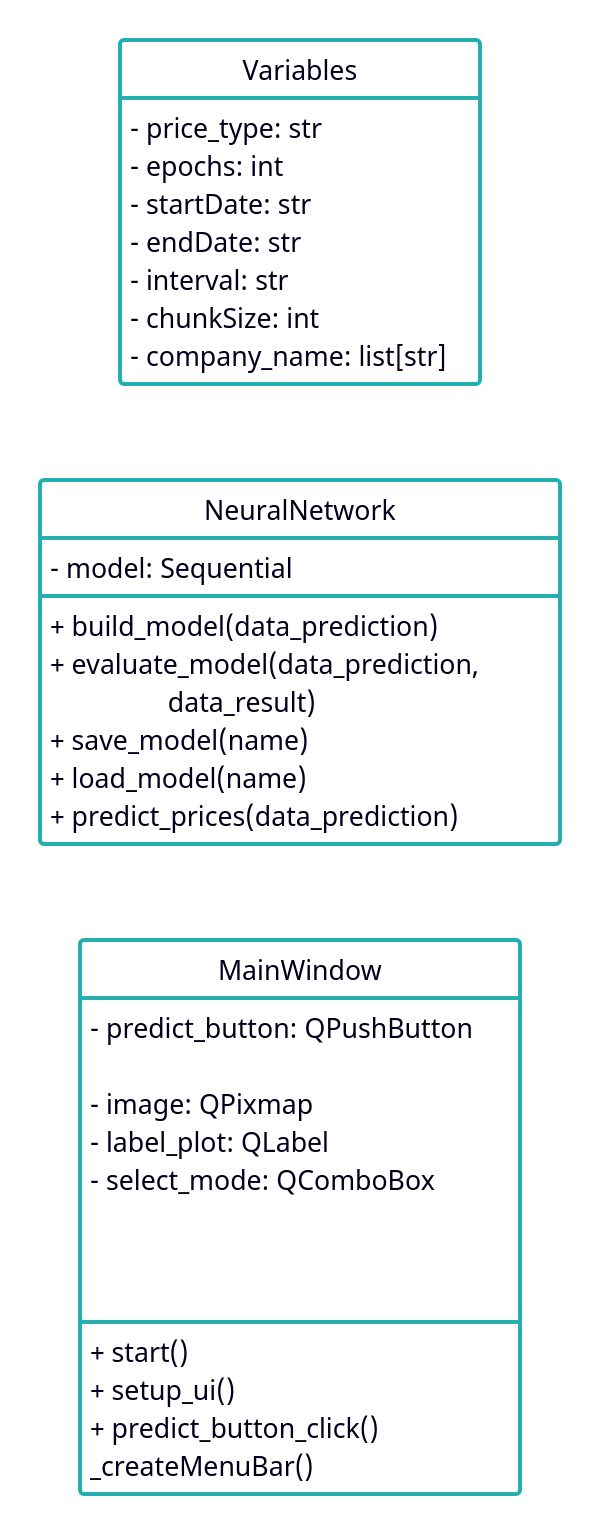
\includegraphics[width=0.6\textwidth]{./graf/UML.png}

  \caption{UML class diagram.}
  \label{fig:label}
  \end{figure} 